% Figure 4 — Masking modes (top) and action-injection variants (bottom)
\documentclass[tikz,border=6pt]{standalone}
% Meta AI / FAIR figure style (I-JEPA / V-JEPA visual language)
% White background, soft pastel rounded blocks, thin borders, sans-serif,
% dashed arrows for EMA / stop-gradient, minimal ink.
\usepackage{amsmath,amssymb}
\usepackage[scaled]{helvet}
\renewcommand{\familydefault}{\sfdefault}
\usepackage{tikz}
\usetikzlibrary{arrows.meta,positioning,fit,calc,backgrounds}

% --- FAIR-like palette -------------------------------------------------------
\definecolor{mblue}{HTML}{BDD7EE}   \definecolor{mblueL}{HTML}{2E75B6}  % context / online encoder
\definecolor{mpink}{HTML}{F8CBAD}   \definecolor{mpinkL}{HTML}{ED7D31}  % target (EMA) encoder
\definecolor{mgreen}{HTML}{C6E0B4}  \definecolor{mgreenL}{HTML}{548235} % predictor
\definecolor{myell}{HTML}{FFE699}   \definecolor{myellL}{HTML}{BF9000}  % actions / conditioning
\definecolor{mgray}{HTML}{F2F2F2}   \definecolor{mgrayL}{HTML}{7F7F7F}  % latents / neutral
\definecolor{mred}{HTML}{F4B8B8}    \definecolor{mredL}{HTML}{C00000}   % loss / dead controls
\definecolor{ink}{HTML}{3B3B3B}

\tikzset{
  every node/.style={font=\sffamily},
  blk/.style={rounded corners=7pt, line width=0.7pt, minimum height=9mm,
              inner xsep=3mm, inner ysep=2mm, align=center, font=\sffamily\small},
  enc/.style ={blk, fill=mblue,  draw=mblueL},
  tgt/.style ={blk, fill=mpink,  draw=mpinkL},
  prd/.style ={blk, fill=mgreen, draw=mgreenL},
  act/.style ={blk, fill=myell,  draw=myellL},
  lat/.style ={blk, fill=mgray,  draw=mgrayL},
  los/.style ={circle, fill=mred, draw=mredL, line width=0.7pt, minimum size=7.5mm,
               font=\sffamily\small, inner sep=0pt},
  lbl/.style ={font=\sffamily\footnotesize, text=ink},
  sub/.style ={font=\sffamily\scriptsize, text=mgrayL},
  ar/.style  ={-{Latex[length=2.4mm]}, line width=0.8pt, draw=ink},
  ema/.style ={-{Latex[length=2.4mm]}, line width=0.8pt, draw=mpinkL, dashed},
  sg/.style  ={ar, postaction={decorate}},  % stop-gradient: annotate with // manually
  cell/.style={draw=mgrayL, line width=0.4pt, minimum size=3.2mm, inner sep=0pt},
  cellm/.style={cell, fill=mblue},          % visible patch
  cellx/.style={cell, fill=mgray},          % masked patch
}
% stop-gradient tick: \sgmark{point}
\newcommand{\sgmark}[1]{\node[rotate=65, font=\footnotesize\bfseries, text=ink] at (#1) {/\!/};}

\begin{document}
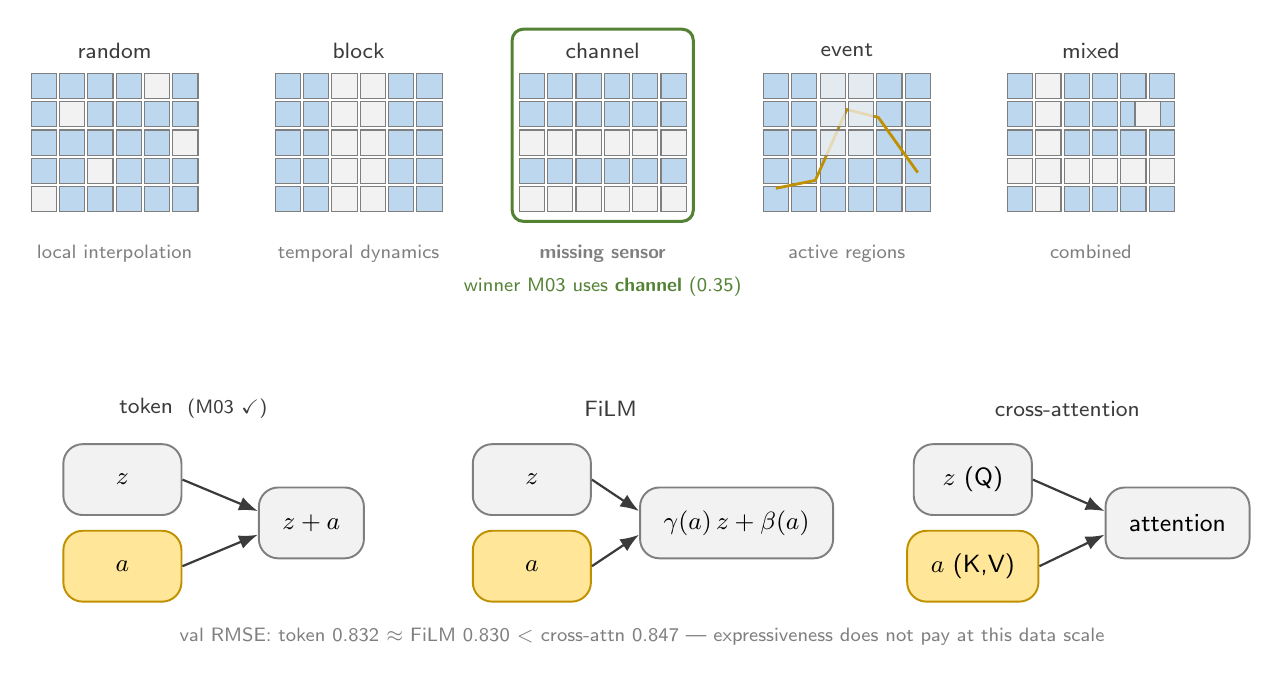
\begin{tikzpicture}

% ============ row 1: masking modes ==========================================
\foreach [count=\k from 0] \name/\capt in {%
  random/local interpolation, block/temporal dynamics,
  channel/\textbf{missing sensor}, event/active regions, mixed/combined}{
  \begin{scope}[shift={(3.1*\k,0)}]
    \node[lbl] at (0.9,0.45) {\name};
    \foreach \i in {0,...,5}{\foreach \j in {0,...,4}{\node[cellm] at (0.36*\i,-0.36*\j) {};}}
    \node[sub, anchor=north, align=center] at (0.9,-1.9) {\capt};
  \end{scope}
}
% masks per mode
\begin{scope}[shift={(0,0)}] % random points
  \foreach \p in {(0.36,-0.36),(1.44,0),(0.72,-1.08),(1.8,-0.72),(0,-1.44)}{\node[cellx] at \p {};}
\end{scope}
\begin{scope}[shift={(3.1,0)}] % temporal block
  \foreach \j in {0,...,4}{\node[cellx] at (0.72,-0.36*\j) {}; \node[cellx] at (1.08,-0.36*\j) {};}
\end{scope}
\begin{scope}[shift={(6.2,0)}] % channel rows
  \foreach \i in {0,...,5}{\node[cellx] at (0.36*\i,-0.72) {}; \node[cellx] at (0.36*\i,-1.44) {};}
  \draw[rounded corners=4pt, draw=mgreenL, line width=1.1pt] (-0.25,0.72) rectangle (2.05,-1.72);
\end{scope}
\begin{scope}[shift={(9.3,0)}] % event
  \draw[draw=myellL, line width=1pt] (0,-1.3) -- (0.5,-1.2) -- (0.9,-0.3) -- (1.3,-0.4) -- (1.8,-1.1);
  \foreach \i in {2,3}{\foreach \j in {0,...,2}{\node[cellx, fill opacity=0.75] at (0.36*\i,-0.36*\j) {};}}
\end{scope}
\begin{scope}[shift={(12.4,0)}] % mixed
  \foreach \j in {0,...,4}{\node[cellx] at (0.36,-0.36*\j) {};}
  \foreach \i in {0,...,5}{\node[cellx] at (0.36*\i,-1.08) {};}
  \node[cellx] at (1.62,-0.36) {};
\end{scope}
\node[sub, text=mgreenL] at (7.1,-2.55) {winner M03 uses \textbf{channel} (0.35)};

% ============ row 2: action injection =======================================
\begin{scope}[shift={(0.4,-4.6)}]
  % token
  \node[lbl] at (1.5,0.5) {token \;{\scriptsize(M03 \checkmark)}};
  \node[lat, minimum width=15mm] (t1) at (0.6,-0.4) {$z$};
  \node[act, minimum width=15mm] (t2) at (0.6,-1.5) {$a$};
  \node[blk, fill=mgray, draw=mgrayL, minimum width=13mm] (t3) at (3.0,-0.95) {$z + a$};
  \draw[ar] (t1.east) -- ($(t3.west)+(0,0.15)$);
  \draw[ar] (t2.east) -- ($(t3.west)+(0,-0.15)$);
\end{scope}

\begin{scope}[shift={(5.6,-4.6)}]
  % FiLM
  \node[lbl] at (1.6,0.5) {FiLM};
  \node[lat, minimum width=15mm] (f1) at (0.6,-0.4) {$z$};
  \node[act, minimum width=15mm] (f2) at (0.6,-1.5) {$a$};
  \node[blk, fill=mgray, draw=mgrayL, minimum width=19mm] (f3) at (3.2,-0.95) {$\gamma(a)\,z + \beta(a)$};
  \draw[ar] (f1.east) -- ($(f3.west)+(0,0.15)$);
  \draw[ar] (f2.east) -- ($(f3.west)+(0,-0.15)$);
\end{scope}

\begin{scope}[shift={(11.2,-4.6)}]
  % cross-attention
  \node[lbl] at (1.8,0.5) {cross-attention};
  \node[lat, minimum width=15mm] (c1) at (0.6,-0.4) {$z$ (Q)};
  \node[act, minimum width=15mm] (c2) at (0.6,-1.5) {$a$ (K,V)};
  \node[blk, fill=mgray, draw=mgrayL, minimum width=17mm] (c3) at (3.2,-0.95) {attention};
  \draw[ar] (c1.east) -- ($(c3.west)+(0,0.15)$);
  \draw[ar] (c2.east) -- ($(c3.west)+(0,-0.15)$);
\end{scope}

\node[sub] at (7.6,-7.0)
  {val RMSE: token 0.832 $\approx$ FiLM 0.830 $<$ cross-attn 0.847 --- expressiveness does not pay at this data scale};

\end{tikzpicture}
\end{document}
